\chapter{Conclusions and possible improvements}
\label{chap:ch6}

In the end, GoogLeNet proved to not be a worthy architecture for the classification of cancer tumors in digital breast tomosynthesis images because of the low accuracy obtained. The highest accuracy obtained was 0.6321 and precision and recall for predicting cancer images were 0.6027 and 0.6087, respectively. I propose a different architecture, maybe DenseNet or ResNet to train and compare the results obtained by GoogLeNet. Additionally, I would increase the length of the dataset even more by including all the slices, keeping in mind the risk that some inputs might overpower others, especially considering the fact that the lowest number of slices an image has in the database is 22, and the highest number is 120.

As for EfficientDet, I am quite happy with the results of the trained model. I would maybe experiment with other types of EfficientDet, from D1 to D5. I do have some concerns, mainly the fact that the test loss seems to slightly increase from epoch to epoch while the train loss decreases. While the CosineAnnealing learning rate decay proved to work well with the model, I would experiment with other types of learning rate decay, such as OneCycle. The test loss obtained was 1.315 and the train loss was 0.2524. I would also experiment with different values for the anchor boxes.

\begin{figure}
    \centering
    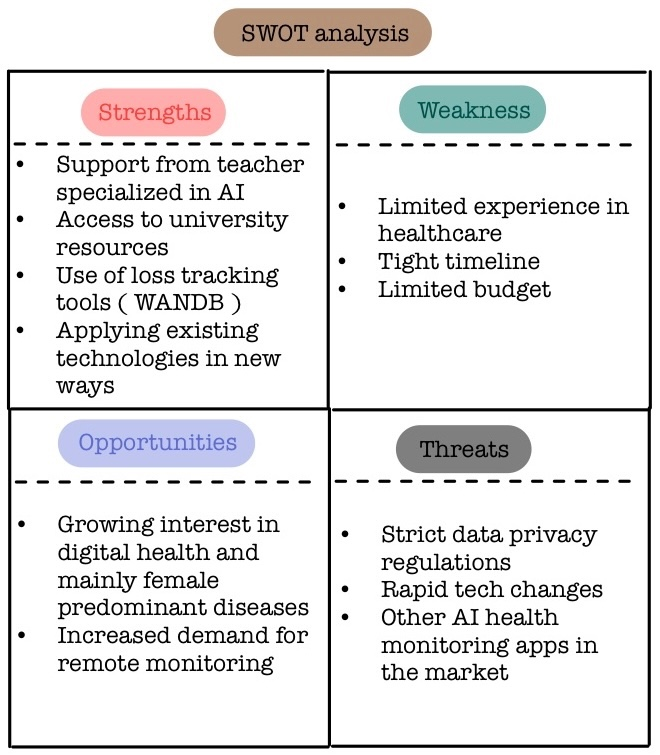
\includegraphics[width=0.5\linewidth]{figures/Figure54.png}
    \caption{SWOT analysis}
    \label{fig:fig44}
\end{figure}